\documentclass[14pt,svgnames,dvipsnames]{beamer}
\usepackage[english]{babel}
\usepackage[misc]{ifsym}
\usepackage[compat=0.2]{TeXnicalities}
\usepackage{%
    fontspec,
    fontawesome,
    mathabx,
    pifont,
    etoolbox,
    xstring,
    listings,
    lstautogobble,
    tikz,
    pgfornament,
    emoji
}

\setsansfont{Yanone Kaffeesatz}[
    UprightFont     = *-Regular ,
    BoldFont        = *-Bold ,
    BoldItalicFont  = *-Bold ,
    BoldSlantedFont = *-Bold ,
    ItalicFont      = *-Light ,
    SlantedFont     = *-Light ,
%    SmallCapsFont   = *-Thin
]

%\setmonofont{Latin Modern Mono Prop}

\input{Preamble/TikzSetup}
\input{Preamble/PieTikz}
\input{Preamble/ListingsSetup}
% Command for section pages
\def\currentsectiontypedefault{lecture}
\def\currentsectiontype{\currentsectiontypedefault}
\newcommand{\session}[2]{%
    \IfStrEqCase{#1}{%
        {lecture}{}%
        {exercise}{}%
        {closing}{}%
    }[\PackageError{}%
        {Wrong first argument to \protect\session\space command.\MessageBreak
         Valid values: lecture, exercise, closing}%
        {}]
    \def\currentsectiontype{#1}
    \setbeamercolor{section page background canvas}{bg=\currentsectiontype}
    \section{#2}
    \def\currentsectiontype{\currentsectiontypedefault} % retore default value
}

% Miscellaneous
\newcommand<>{\tc}[2]{\textcolor#3{#1}{#2}}
\newcommand{\myCopyright}{\raisebox{-7pt}{\large\copyright}}
\newcommand{\yes}{\parbox{5mm}{\,\textcolor{ForestGreen}{\ding{51}}}}
\newcommand{\inPr}{\parbox{5mm}{\,\textcolor{Gray}{\faCog}}}
\newcommand{\no}{\parbox{5mm}{\,\textcolor{OrangeRed}{\ding{55}}}}
%\pgfkeys{/beamer/overlayarea/show frame}

% Command to vertically center emoji
\newsavebox{\emojibox}
\newcommand{\Emoji}[2][\normalsize]{%
    \sbox{\emojibox}{#1\emoji{#2}}%
    \raisebox{-0.33\ht\emojibox}{\usebox{\emojibox}}%
}


% Do a square with number inside as enumerate environment does
\newcommand{\MakeEnumerateBox}[1]%
{%
    \hbox{%
      \usebeamerfont*{item projected}%
      \usebeamercolor[bg]{item projected}%
      \vrule width2.25ex height1.85ex depth.4ex%
      \hskip-2.25ex%
      \hbox to2.25ex{%
        \hfil%
        \color{fg}#1%
        \hfil}%
    }%
}

%Tikz group of commands to make a pyramid layer
\newcommand{\pyramidLayer}[6][]{%
    \pgfmathsetmacro{\Thickness}{#3}
    \pgfmathsetmacro{\Long}{#4}
    \pgfmathsetmacro{\Short}{#4-0.5*#3}
    \path coordinate (middleUpperRight) at ($(#2)+(0,\Thickness)+(30:0.5*\Short)$)
          coordinate (middleLowerRight) at ($(#2)+(30:0.5*\Long)$)
          coordinate (upperRight) at ($(#2)+(0,\Thickness)+(30:\Short)$)
          coordinate (lowerRight) at ($(#2)+(30:\Long)$);
    \draw[fill=#5!50] ($(#2)+(0,\Thickness)+(30:\Short)$)  -- ++(210:\Short) -- ++(270:\Thickness) -- ++(30:\Long) -- cycle;
    \draw[fill=#5!20] ($(#2)+(0,\Thickness)+(150:\Short)$)  -- ++(330:\Short) -- ++(270:\Thickness) -- ++(150:\Long) -- cycle;
    \draw[fill=#5]    ($(#2)+(0,\Thickness)$) -- ++(30:\Short) -- ++(150:\Short) -- ++(210:\Short) -- cycle;
    \node[font=\small] at ($(middleUpperRight)!0.5!(middleLowerRight)$) {\rotatebox{30}{#6}};
    \node[text=#5, anchor=west] at ($(upperRight)!0.5!(lowerRight)+(0.5,0)$) {#1};
}

\graphicspath{{Figures/}}
% Compile with or without links to TOC
\newif\ifAddLinkToTOC
\AddLinkToTOCtrue

% Command to define beamer template for TOC. This is basically identical to the beamer template
% except for what colours are used. The used colors are those defined later in this file: either
% lecture, exercise or closing.
\newcommand{\installTOCbeamertemplate}[1]{%
    \defbeamertemplate*{#1 section in toc}{default}{%
        \leavevmode\leftskip=1.75ex%
        \llap{%
            \usebeamerfont*{section number projected}%
            \usebeamercolor[bg]{#1 section}%
            \vrule width2.25ex height1.85ex depth.4ex%
            \hskip-2.25ex%
            \hbox to2.25ex{\hfil\usebeamercolor[fg]{#1 section}\inserttocsectionnumber\hfil}}%
        \kern1.25ex\usebeamercolor[bg]{#1 section}\inserttocsection\par%
    }
    \defbeamertemplate*{#1 section in toc shaded}{default}[1][20]
        {\begin{colormixin}{##1!parent.bg}\usebeamertemplate{#1 section in toc}\end{colormixin}\unskip}
}

\mode<presentation>
{
    \usetheme{Z02}
    \defbeamertemplate{footline}{Empty}{}
    \setbeamersize{text margin left=5mm,text margin right=5mm}
    \setbeamerfont{title}{size=\huge}
    \setbeamerfont{subtitle}{size=\LARGE}
    %\setbeamerfont{section title}{size=\Huge}
    %Add a link to table of content on frames with a footline
    \addtobeamertemplate{footline}{}{%
        \ifAddLinkToTOC%
            \begin{tikzpicture}[remember picture,overlay]
                %xelatex needs \XeTeXLinkBox, won't create a link unless it
                %finds text --- rules don't work without \XeTeXLinkBox.
                %Still builds correctly with pdflatex and lualatex
                \node[anchor=south east, inner sep=3pt, font=\scriptsize] at (current page.south east) {\hyperlink{toc}{\XeTeXLinkBox{\emoji{blue-book}}}};
            \end{tikzpicture}%
        \fi%
    }%
    % New templates to change square and title color in TOC
    \colorlet{lecture}{BGDARK}
    \colorlet{exercise}{PS}
    \colorlet{closing}{PQ}
    \setbeamercolor{lecture section}{bg=lecture, fg=BGLIGHT}
    \setbeamercolor{exercise section}{bg=exercise, fg=BGLIGHT}
    \setbeamercolor{closing section}{bg=closing, fg=BGLIGHT}
    \installTOCbeamertemplate{lecture}
    \installTOCbeamertemplate{exercise}
    \installTOCbeamertemplate{closing}
    \setbeamercolor{subsection page background canvas}{bg=PB}
}

\makeatletter
\AtBeginSection[]% <- Empty optional argument, do nothing for \section*
{%
    \ifnum\beamer@tocsectionnumber>0%
        \begin{frame}[plain, noframenumbering]{}
             \sectionpage
        \end{frame}
    \fi
}
\AtBeginSubsection[]% <- Empty optional argument, do nothing for \subsection*
{%
    \ifnum\beamer@tocsectionnumber>0%
        \begin{frame}[plain, noframenumbering]{}
             \subsectionpage
        \end{frame}
    \fi
}
\makeatother

%Append code to put license and GitHub profile to titlepage
\newcommand{\GitHubAuthors}[1]{
    \def\insertGitHubAuthors{#1}
}
\appto\titlepage{%
    \begin{tikzpicture}[remember picture, overlay]
        \node[anchor=south, inner ysep=0pt] (license) at ($(current page.south)+(0mm,3mm)$)
        {
\includegraphics[width=10mm]{CC-BY}};
        \node[anchor=south, font=\small, text=BGLIGHT] (Axel) at (license.north)
        {\insertGitHubAuthors};
    \end{tikzpicture}
}

%===============================================================%
\title{Clean software development}
\titlegraphic{$\stackrel{
\includegraphics[width=24mm]{Logo-CRC}}{
\includegraphics[width=24mm]{Logo-HGS-HIRe}}$}
%===============================================================%


% The following code has been taked from the beamer class beamerbasesection.sty file and changed
% so that the  \addtocontents{toc} adds now a 6th argument to the .toc file, which is the color
% to be used in the TOC. This is the command that among others is adding lines to the .toc file
% which is later used to typeset the TOC.
%
% NOTE: The default \section command still works and uses the lecture type as this is set as
%       default in the \session command.
\makeatletter
\long\def\beamer@section[#1]#2{%
    \beamer@savemode%
    \mode<all>%
    \ifbeamer@inlecture
    \refstepcounter{section}%
    \ifblank{#2}%
    {\long\def\secname{#1}\long\def\lastsection{#1}}%
    {\global\advance\beamer@tocsectionnumber by 1\relax%
        \long\def\secname{#2}%
        \long\def\lastsection{#1}%
        \addtocontents{toc}{\protect\beamer@sectionintoc{\the\c@section}{#2}{\the\c@page}{\the\c@part}%
            {\the\beamer@tocsectionnumber}{\currentsectiontype}}}% <---- CHANGED
    {\let\\=\relax\xdef\sectionlink{{Navigation\the\c@page}{\noexpand\secname}}}%
    \beamer@tempcount=\c@page\advance\beamer@tempcount by -1%
    \addtocontents{nav}{\protect\headcommand{\protect\beamer@sectionpages{\the\beamer@sectionstartpage}{\the\beamer@tempcount}}}%
    \addtocontents{nav}{\protect\headcommand{\protect\beamer@subsectionpages{\the\beamer@subsectionstartpage}{\the\beamer@tempcount}}}%
    \ifblank{#1}{}{%
        \addtocontents{nav}{\protect\headcommand{\protect\sectionentry{\the\c@section}{#1}{\the\c@page}{\secname}{\the\c@part}}}%
    }%
    \beamer@sectionstartpage=\c@page%
    \beamer@subsectionstartpage=\c@page%
    \def\insertsection{\expandafter\hyperlink\sectionlink}%
    \def\insertsubsection{}%
    \def\insertsubsubsection{}%
    % Deal with a defective patch in metropolis theme
    \def\insertsectionhead{\hyperlink{Navigation\the\c@page}{#1}}%
    \edef\insertsectionhead{\noexpand\hyperlink{Navigation\the\c@page}{\unexpanded{#1}}}%
    \def\insertsubsectionhead{}%
    \def\insertsubsubsectionhead{}%
    \def\lastsubsection{}%
    \Hy@writebookmark{\the\c@section}{\secname}{Outline\the\c@part.\the\c@section}{2}{toc}%
    \hyper@anchorstart{Outline\the\c@part.\the\c@section}\hyper@anchorend%
    \ifblank{#2}{\beamer@atbeginsections}{\beamer@atbeginsection}%
    \fi%
    \beamer@resumemode}%

% The following code has also been taked from the beamer class beamerbasetoc.sty file and changed
% in a couple of places:
%   1. The command takes 6 arguments
%   2. The \beamer@tocact command is used with a template name that depends on the 6th argument
\def\beamer@sectionintoc#1#2#3#4#5#6{% <--- CHANGED
    \ifnum\c@tocdepth>0%
    \ifnum#4=\beamer@showpartnumber%
    {
        \beamer@saveanother%
        \gdef\beamer@todo{}%
        \beamer@slideinframe=#1\relax%
        \expandafter\only\beamer@tocsections{\gdef\beamer@todo{%
                \beamer@tempcount=#5\relax%
                \advance\beamer@tempcount by\beamer@sectionadjust%
                \ifnum\beamer@tempcount>0
                \edef\inserttocsectionnumber{\the\beamer@tempcount}%
                \else
                \def\inserttocsectionnumber{}%
                \fi%
                \def\inserttocsection{\hyperlink{Navigation#3}{#2}}%
                \beamer@tocifnothide{\ifnum\c@section=#1\beamer@toc@cs\else\beamer@toc@os\fi}%
                {%
                    \ifbeamer@pausesections\pause\fi%
                    \ifx\beamer@toc@ooss\beamer@hidetext
                    \vskip1.5em
                    \else
                    \vfill
                    \fi
                    {%
                        \hbox{\vbox{%
                                \def\beamer@breakhere{\\}%
                                \beamer@tocact{\ifnum\c@section=#1\beamer@toc@cs\else\beamer@toc@os\fi}{#6 section in toc}}}%  <--- CHANGED
                        \par%
                    }%
                }%
            }%
        }%
        \beamer@restoreanother%
    }
    \beamer@todo%
    \fi\fi%
}
\makeatother











\newcommand{\nconf}{N_{\text{conf}}}
\newcommand{\Nconf}{\nconf}


%===================%
\subtitle{Day 4}
\author{David A. Clarke}
\institute{Z02~--~Software Development Center}
\titlepagelogo{
\includegraphics[width=24mm]{Logo-FRA}}
\GitHubAuthors{\href{https://github.com/clarkedavida}{\faGithub\,clarkedavida}}
\date{9 October 2025}
%===================%

\begin{document}
    %-------------------------------%
%  Author: Alessandro Sciarra   %
%    Date: 26 Jun 2025          %
%-------------------------------%

%~~~~~~~~~~~~~~~~~~~~~~~~~~~~~~~~~~~~~~~~~~~~%
\PrepareURLsymbol[PB]
%~~~~~~~~~~~~~~~~~~~~~~~~~~~~~~~~~~~~~~~~~~~~%
\begin{frame}[plain,noframenumbering]
    \titlepage
\end{frame}
%~~~~~~~~~~~~~~~~~~~~~~~~~~~~~~~~~~~~~~~~~~~~%
\begin{frame}[label=toc,plain,noframenumbering]{Topics of the day}
    \begin{columns}
        \hfill
        \begin{column}{.55\textwidth}
            \hspace*{4mm}
            \begin{minipage}[0.5\textheight]{\textwidth}
                \tableofcontents[sections={1-4}]
            \end{minipage}
        \end{column}
        \hfill
        \begin{column}{.4\textwidth}
            \begin{minipage}[0.5\textheight]{\textwidth}
                \tableofcontents[sections={5-}, hideallsubsections]
            \end{minipage}
        \end{column}
        \hfill
    \end{columns}
    \vspace{2mm}
    \begin{varblock}{quote}[\textwidth]{Cross checking}
        \normalfont\small
        Today the goal is to learn and practice several strategies
        to validate and clean data.\\
         We will write our own code from scratch!
    \end{varblock}
\end{frame}
%~~~~~~~~~~~~~~~~~~~~~~~~~~~~~~~~~~~~~~~~~~~~%

    \session{lecture}{Motivation}
    
%===================================================================================================%


\frame{\frametitle{Objectives}
\centering
We are going to \textbf{learn good practices
curating scientific data} \\ through a small
data analysis project.\\[5mm]

Everything I present
here I learned by watching excellent scientists.\\ This
is my attempt to emulate them.\\[5mm] 

I try to keep lecture roughly self-contained.\\[5mm]

\textbf{Please interrupt at any time!}
}



\frame{\frametitle{Testing and validation}

\begin{itemize}
\item Testing: Carrying out \textbf{checks of functionality
and correctness} of code
\item Validation: Testing that focuses in particular
on the \textbf{scientific correctness} of code
\item As always, driven by \textbf{falsification principle}
\end{itemize}
\vspace{5mm}

My personal tower of priorities:
\begin{enumerate}
\item Code output is \textbf{consistent}
\begin{itemize}
\item Self-consistency % code does not produce two contradictory numbers
\item Consistent with what we ``know" % i.e. consistent with physics knowledge
\end{itemize}
\item Code is \textbf{clean} and \textbf{understandable}
% understandable is not really up to you. if someone else uses your code
% and tells you they don't understand it, that is generally your fault!
\item Code is \textbf{efficient}
\end{enumerate}
\vspace{5mm}

Everything else (elegant, clever, cute, etc.) is fluff.
}



    \session{lecture}{Validating data}
    
%===================================================================================================%


\frame{\frametitle{Testing strategies}
Here are some ideas to check consistency of code output.
I think of them as Cross Checks.
Some are the \textbf{same checks you do in physics}.
What I use most commonly (no particular order, not exhaustive, not disjoint):
\begin{enumerate}
\item Compare against trusted result
% can be from literature, another code base, etc 
\item Compare with an analytic calculation
\item Compute a result multiple ways
\item Check for consistency between observables
% for example if one obs is the derivative of the other,
% that constrains how they must be related
\item Check known properties
% probabilities in [0,1]; 2d ising magnetization monotonic in T
\item Verify independence of hyperparameters
% dependence on jackknife bin size? solve tolerance? 
\end{enumerate}
}

\frame{\frametitle{CC1: Compare against trusted result}
\begin{itemize}
\item Often a starting point: \textbf{reproduce something}
% e.g. if you are implementing something new following the method
% of a paper, start by reproducing what's in that paper
\item Danger: you \textbf{assume other calculation is correct}
\begin{itemize}
\item Has the result already been reproduced?
\item You could apply some Cross Checks to the trusted result
\item If you are unsure about trusted result,
\textbf{blinding} can help against human bias: 
\begin{enumerate}
\item Let $r\in[-R,R]$ unknown to you 
\item Rescale your observable by $r$
\item Remove $r$ when you are confident in your calculation
\end{enumerate}
\end{itemize}
\item Can test against your old results to \textbf{ensure stability}
\begin{itemize}
\item Some of your unit tests could work this way
\end{itemize}
\end{itemize}
% Example of CMD? Or maybe the electron whatever thing
}

\frame{\frametitle{CC2: Compare with an analytic calculation}
\begin{itemize}
\item Simple test case \textbf{calculable by hand}
\item Known result from theory
\end{itemize}
% diff_deriv
}


\frame{\frametitle{CC3: Compute a result multiple ways}
There's usually more than one way to solve a problem
\begin{itemize}
\item Check optimized implementation against easy-to-understand one
\item Test different algorithms against each other
\item Test different models against each other
\end{itemize}
% Example of correlator class in GPU
% Different integration techniques give same result
}


\frame{\frametitle{CC4: Check for consistency between observables}
Two observables may be constrained by relationships between them.
Design tests that ensure observables obey these known constraints.
% Acceleration/velocity?
% What kinds of checks did Frithjof do?
% Maybe one of your checks from material params
}


\frame{\frametitle{CC5: Check known properties}
Depending on an observable's interpretation, you may already
know some properties it must have. Test them! Examples:
\begin{enumerate}
\item is your covariance matrix positive semidefinite?
\item is your unitary matrix actually unitary?
\item is your RHMC reversible?
\item is your probability between 0 and 1?
\end{enumerate}
}


\frame{\frametitle{CC6: Verify independence of hyperparameters}
\begin{itemize}
\item Parameter: Directly \textbf{model-relevant} number
\begin{itemize}
\item Temperature, volume, particle mass, coupling constant
\item Fit parameters 
\end{itemize}
\item Hyperparameter: Needed \textbf{only for computational strategy}
\begin{itemize}
\item Jackknife bins, bootstrap samples
\item Initial guess of a fitter
\item Max iterations, solve tolerance, CNN kernel size 
\end{itemize}
\item Often only independent of hyperparameter \textbf{in some region}
\begin{itemize}
\item Number of jackknife bins until error bar plateaus 
\item Initial guesses leading to reasonable $\chi^2/{\rm d.o.f.}$
\end{itemize}
\end{itemize}
}




    \session{lecture}{Cleaning data}
    
%===================================================================================================%

\frame{\frametitle{The issue}
Eventually you will come across data from many different
people/groups. Possible problems:
\begin{itemize}
\item Different conventions
\item Different data formats
\item Duplicate entries
\item Damaged/lost/unlabelled files
\end{itemize}
\vspace{5mm}
\centering
% FAIR paper
We are in an era where significant effort is put into
ensuring \\ data can be \textbf{readily used and reproduced}.
}

\frame{\frametitle{Practical goals for your own work}
What will save you a lot of pain:
\begin{itemize}
\item You know where your data is
\item You can read your old data
\item Sufficient metadata to know what your data means
\item You can tell if your data got damaged 
\item Your data is homogeneous and/or well organized
\end{itemize}
}


\frame{\frametitle{Toward these goals}
\begin{enumerate}
\item Bring input data into common format
% Example: Graduate student asks me to analyze data,
% format different between data sets
\begin{itemize}
\item Makes it easier to write/debug scripts
\item Helps next person using your work
\item Opportunity for cross-checks
\end{itemize}
\item Stay consistent with conventions
\item Try to use already-existing data structures (e.g.
\texttt{yaml} or \texttt{csv})
\begin{itemize}
\item Everyone can leverage already-existing tools
\item Lots of information about format structure 
\end{itemize}
\item Label your columns
\item Add \texttt{README.md} for supplemental information
\end{enumerate}
}



    \session{lecture}{Plotting data}
    
%===================================================================================================%

\begin{frame}[fragile]{Visualizing data for Cross Checks}
\begin{itemize}
\item Visualizations help understanding
\item You will be plotting in your papers
\item Gives further opportunities for cross checks!
\end{itemize}
\begin{onlyenv}<1>
\begin{varblock}{example}[\textwidth]{Ex: Are these data consistent?}
\small
\begin{verbatim}
#          t [ms]      speed [m/s]    accel [m/s^2]
   0.00000000e+00   0.00000000e+00   0.00000000e+00
   1.00000000e+00   5.00000000e-01   1.00000000e+00
   2.00000000e+00   2.00000000e+00   2.00000000e+00
   3.00000000e+00   4.50000000e+00   3.00000000e+00
   4.00000000e+00   8.00000000e+00   4.00000000e+00
   5.00000000e+00   1.25000000e+01   5.00000000e+00
\end{verbatim}
\end{varblock}
\end{onlyenv}
\end{frame}

% maybe work out pressure and baryon number example:
% - used webplotdigitizer to get HRG data from hotqcd
% - wrote test to compare pressure against that
% - plot pressure and n_B vs mu_B to see if it makes sense

\begin{frame}{Ex: Are these data consistent?}
\centering
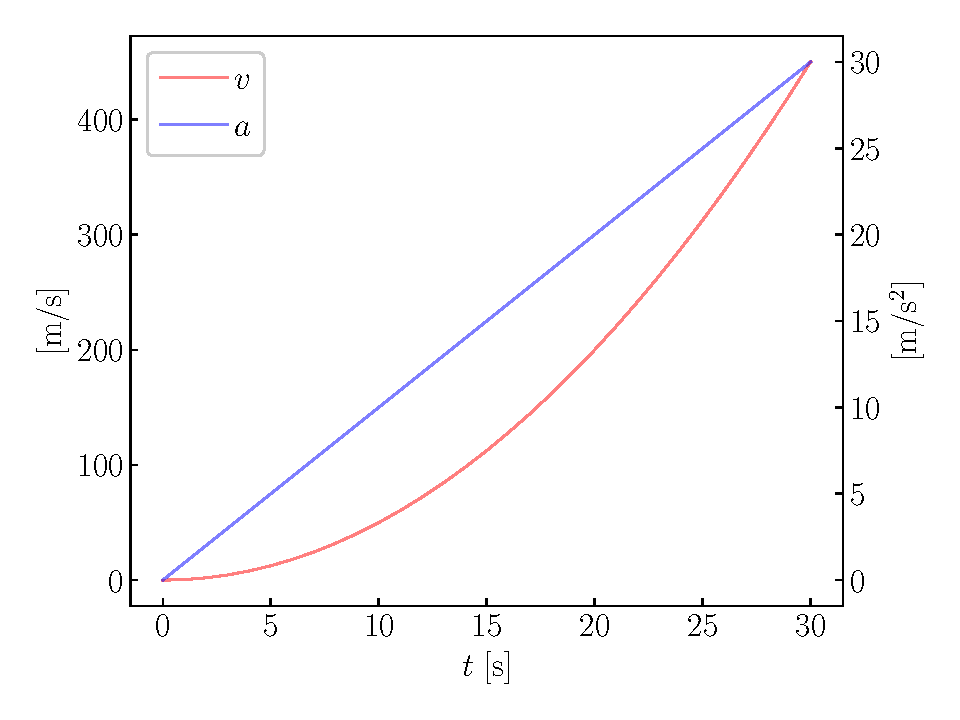
\includegraphics[width=0.8\textwidth]{dataAnalysis/speed_accel.pdf}
\end{frame}


    \session{lecture}{2D Ising model (I)}
    
%===================================================================================================%

\begin{frame}{The 2-$d$ Ising model}
We are going to practice data cleaning and validation in the context
of the 2-$d$ Ising model, a model for a magnet.
\begin{itemize}
\item One of the simplest magnet models
\item Analytically solvable (Cross Check 2)
\item Applications to phase transitions
\item Pedagogical for phase transitions
\end{itemize}
\end{frame}

\begin{frame}{The 2-$d$ Ising model}
\centering
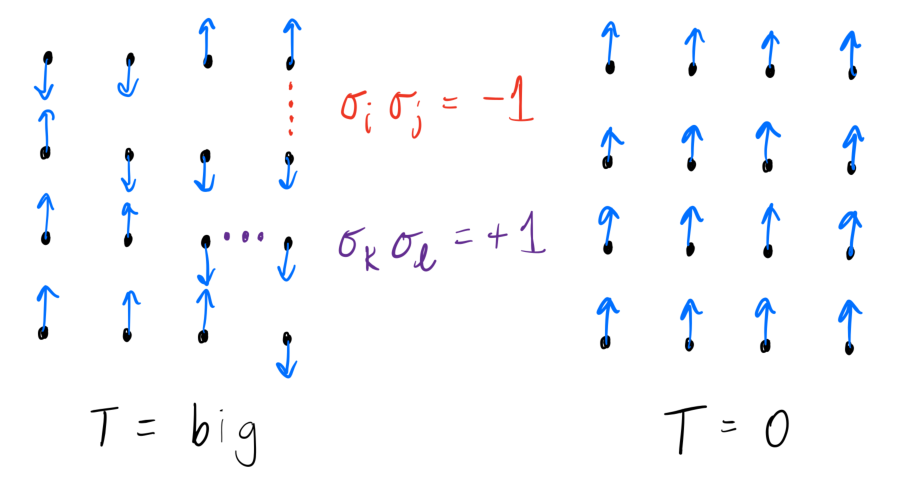
\includegraphics[width=0.8\textwidth]{dataAnalysis/isingModel.pdf}
$$
H=-J\sum_{\langle ij\rangle} \sigma_i \sigma_j
~~~~~ ~~~~~ ~~~~~
\textrm{pr}(C)\sim e^{-H(C)/T}
$$
\end{frame}

\begin{frame}{Solving Ising with MCMC}
Common strategy: Generate $\nconf$ configurations randomly, then
estimate expectation value of observable $X$
$$
  \bar{X}=\frac{1}{\nconf}\sum_{i=1}^{\nconf} X_i
$$
Each $X_i$ measured on conf $C_i$ from Markov Chain
$$
  C_0\to C_1\to C_2\to...
$$
\end{frame}

% unbiased variance
% assumes uncorrelated data, but they are actually correlated
% can show variance of correlated data is larger than if one
%  had estimated it assuming independence; difference is integrated
%  autocorrelation time
% can therefore think of tau_int as factor between effectively
%  independent configurations and actual number of configurations
% can use this to correct error or to guide strategies to prune data
% note that correct estimate of tau_int demands requires preserving
%  Monte Carlo order!

% an observable you might want to estimate: magnetization
% why? It's the "order parameter" --> properties of |m|/site

% DESCRIBE TASK
% open-ended question: what kind of checks can you build in
%  while you're cleaning the data?

    \session{lecture}{Estimating uncertainties}
    
%===================================================================================================%

\begin{frame}{Reminder: Mean and uncertainty}
    \vspace{-3mm}
    \begin{varblock}{example}[0.9\textwidth]{$C_0\to C_1\to C_2\to...$}
        Mean and variance estimated via
        \vspace{-3mm}
        $$
          \bar{X}=\frac{1}{\nconf}\sum_{i=1}^{\nconf} X_i
        ~~~~ ~~~~ ~~~~
        \sigma^2=\frac{1}{\nconf-1}\sum_{i=1}^{\nconf}\left(X_i^2-\bar{X}^2\right)
        $$
    \end{varblock}
    \begin{varblock}{alert}[\textwidth]{Problem:}
        $C_i$ is generated as deformation of $C_{i-1}$. Hence $X_i$ and
        $X_{i-1}$ are correlated: %, and one can show
        \begin{equation*}
            \sigma^2_X
            = \tau_{\textrm{int}}\frac{\sigma^2}{\nconf}
            \neq \frac{\sigma^2}{\nconf}
        \end{equation*}
        with \textbf{integrated autocorrelation time} $\tau_{\textrm{int}}$.
    \end{varblock}
\end{frame}

\begin{frame}{Autocorrelation}
    \begin{varblock*}{alert}[0.93\textwidth]{}
        The relation
        $$
        \sigma^2_X
        = \tau_{\textrm{int}}\frac{\sigma^2}{\nconf}
        $$
        shows there are effectively $\nconf/\tau_{\textrm{int}}$ independent
        measurements.
    \end{varblock*}
    \begin{varblock*}{example}[0.88\textwidth]{Solutions?}
        Let $M\in\mathbb{N}$ s.t. $M>\tau_{\textrm{int}}$
        \begin{itemize}
            \item \textbf{Decimation}: Keep only measurements $X_0$,
            $X_M$, $X_{2M}$, etc.
            \item \textbf{Binning}: Construct $Y_0$ as average over first $M$ measurements,
            $Y_1$ as average over the next $M$, etc.
        \end{itemize}
    \end{varblock*}
\end{frame}

\begin{frame}{Tricky uncertainties}
\begin{columns}
    \begin{column}{0.9\textwidth}
        Given $\{X_1,...,X_N\}$. Consider some function $f(X)$
        \begin{itemize}
        \item How to get unbiased estimate of $\langle f(X)\rangle$?
        \item What if $f$ is too complicated for error propagation?
        \end{itemize}

        \vspace{5mm}

        $$
        \chi\equiv\frac{V}{T}\left(\langle|m|^2\rangle-\langle|m|\rangle^2\right)
        $$
        Susceptibility $\chi$ is already a variance. How to get its uncertainty?\\[5mm]

        Can tackle both kinds of problems using \textbf{resampling}
    \end{column}
\end{columns}
\end{frame}


\begin{frame}{Resampling: Jackknife}
\centering
Create $N$ new samples by dropping a measurement from old sample\\[5mm]
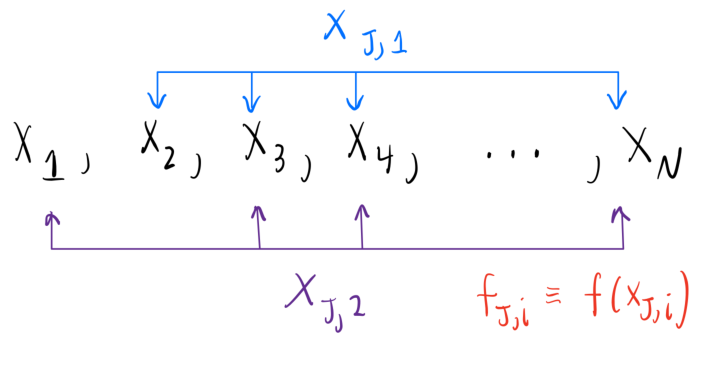
\includegraphics[width=0.8\textwidth]{dataAnalysis/jackknife.pdf}
\end{frame}


\begin{frame}{Resampling: Jackknife}
\textbf{Jackknifed} data are defined by
$$
  X_{J,i}\equiv\frac{1}{N-1}\sum_{j\neq i}X_j
$$
Construct asymptotically unbiased \textbf{jackknife estimator}
for the mean $\bar{f}_J$:
$$
  \bar{f}_J\equiv\frac{1}{N}\sum_{i=1}^N f_{J,i}
  ~~~~ ~~~~ ~~~~ f_{J,i}\equiv f(X_{J,i})
$$
The jackknife estimator for the
variance of $\bar{f}_J$ is
$$
  \bar\sigma^2_{f_J}=\frac{N-1}{N}\sum_{i=1}^N(f_{J,i}-\bar{f}_J)^2
$$
\end{frame}


\begin{frame}[fragile]{Resampling: Jackknife}
\begin{varblock}{example}[\textwidth]{Ex: Susceptibility}
$
\chi\equiv(V/T)\left(\langle|m|^2\rangle-\langle|m|\rangle^2\right)
$

\vspace{2mm}
Can be handled by thinking of $|m|^2$ and $|m|$
as two separate variables $x$ and $y$. Alternatively can think
of susceptibility function $f$ as
\vspace{2mm}

$
f(m)\,\propto\, \langle|m|^2\rangle-\langle|m|\rangle^2
$

\vspace{2mm}

Either way, the important feature is $|m|^2$ and $|m|$\\
\textbf{are divided into the exact same bins}.

\vspace{6mm}

\begin{lstlisting}[style=mypython]
def susc(m,V,T):
    return (V/T)*( np.mean(m**2) - np.mean(m)**2 )

chi, chi_err = jackknife(susc, M, args=(V,T), numb_blocks=20)
\end{lstlisting}
\end{varblock}
\end{frame}


\begin{frame}{Resampling: Bootstrap}
\centering
Create $N_{\textrm{boot}}$ new samples by drawing \\ with replacement
from original sample $N$ times \\[5mm]
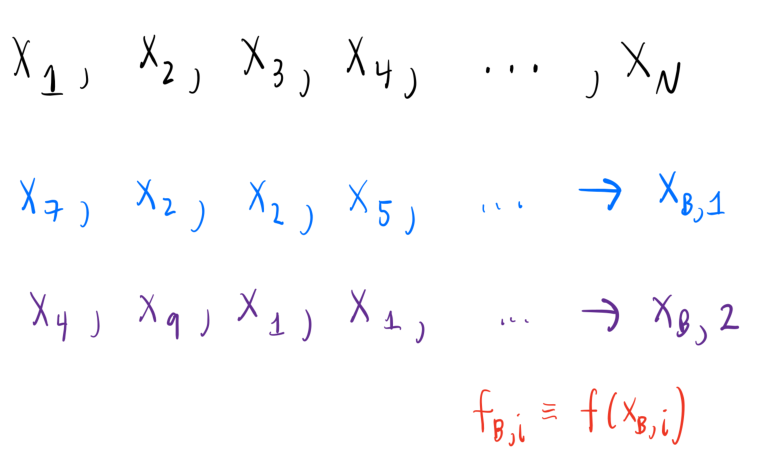
\includegraphics[width=0.8\textwidth]{dataAnalysis/bootstrap.pdf}
\end{frame}

\begin{frame}{Resampling: Bootstrap}
Data are {\it bootstrapped} as
\vspace{-4mm}
$$
X_{B,i}\equiv\frac{1}{N}\sum_{j=1}^Nn_{ij}X_j
$$
where $X_j$ appears $n_{ij}$ times in bin $i$.
As with jackknife, the \textbf{bootstrap estimator}
of the mean $\bar{f}_B$ is
\vspace{-3mm}

$$
  \bar{f}_B\equiv\frac{1}{N_{\textrm{boot}}}\sum_{i=1}^{N_{\textrm{boot}}} f_{B,i},
~~~~ ~~~~ ~~~~
f_{B,i}\equiv f(X_{B,i})
$$
The bootstrap estimator for the variance of $\bar{f}_B$ is simply
$$
  \bar\sigma^2_{f_B}=\frac{1}{N_{\textrm{boot}}-1}
\sum_{i=1}^{N_{\textrm{boot}}}(f_{B,i}-\bar{f}_B)^2.
$$
\end{frame}

\begin{frame}{Synthesis}
    \begin{varblock*}{}[0.82\textwidth]{When some function $f$ of data $X_i$ from a time series}
        \begin{enumerate}
        \item Bin the $X_i$ into $X_{B,j}$
        \item Resample the $X_{B,j}$ (can be combined with first step)
        \item Compute $f(X_{B,j})$ in each resample
        \end{enumerate}
    \end{varblock*}
    \begin{center}
        \Emoji[\Huge]{raised-hands}
    \end{center}
    \vspace{-3mm}
    \begin{varblock}{alert}[0.7\textwidth]{Question for you}
        \large\textbf{How can we validate these results?}
    \end{varblock}
\end{frame}

%    \session{lecture}{Fitting with priors}
%    \input{Slides/dataAnalysis/fit}
%    \session{lecture}{Bayesian model averaging}
%    \input{Slides/dataAnalysis/BMA}
    \session{lecture}{2D Ising model (II)}
    
%===================================================================================================%

\begin{frame}{Extracting $T_c$}
The \textbf{Binder cumulant} is defined as
$$
B\equiv1-\frac{\langle m^4\rangle}{3\langle m^2\rangle^2}
$$
\begin{itemize}
\item $B$ computed at different $L$ will cross at $T_c$
\item $B=0$ for $T\gg T_c$; $B=2/3$ for $T\ll T_c$
\item Easier to get $T_c$ than using $\chi$
\end{itemize}
\end{frame}

\end{document}
